\documentclass[11pt]{article}
\usepackage[margin=1in]{geometry}
\usepackage{fontspec}
\usepackage{booktabs}
\usepackage{longtable}
\usepackage{array}
\usepackage{float}
\usepackage{graphicx}
\usepackage[font=small,labelfont=bf]{caption}
\usepackage{natbib}
\usepackage{xurl}
\usepackage[hidelinks]{hyperref}
\usepackage{setspace}
\setstretch{1.15}
\graphicspath{{../figs/}}
% Generated by scripts/tables.R; do not edit.
\newcommand{\nAlumniMc}{174}
\newcommand{\nAlumniScale}{160}
\newcommand{\nStaffMc}{87}
\newcommand{\nStaffScale}{90}
\newcommand{\nMarchMc}{557}
\newcommand{\nMarchScale}{502}
\newcommand{\nJulyMc}{246}
\newcommand{\nJulyMedia}{237}
\newcommand{\nJulyScale}{267}
\newcommand{\nTotal}{2,320}
\newcommand{\staffRepMc}{17\%}
\newcommand{\staffRepScale}{8\%}
\newcommand{\nPropositions}{30}
\newcommand{\nDropped}{7}
\newcommand{\nMarchPropositions}{20}
\newcommand{\shareKnowledge}{36\%}
\newcommand{\shareMisinformation}{8\%}
\newcommand{\shareMiddle}{56\%}
\newcommand{\shareMidpoint}{16\%}
\newcommand{\julySkipMin}{4\%}
\newcommand{\julySkipMax}{43\%}
\newcommand{\muslimMedia}{27\%}
\newcommand{\muslimMc}{17\%}
\newcommand{\muslimScale}{4\%}
\newcommand{\illegalMedia}{38\%}
\newcommand{\illegalMc}{23\%}
\newcommand{\illegalScale}{3\%}
\newcommand{\fraudMedia}{35\%}
\newcommand{\fraudMc}{16\%}
\newcommand{\fraudScale}{7\%}
\newcommand{\deficitMedia}{80\%}
\newcommand{\deficitMc}{58\%}
\newcommand{\deficitScale}{29\%}
\newcommand{\pooledStrict}{8}
\newcommand{\pooledStrictLower}{6}
\newcommand{\pooledStrictUpper}{11}
\newcommand{\pooledLenient}{4}
\newcommand{\julyStrict}{13}
\newcommand{\julyStrictLower}{10}
\newcommand{\julyStrictUpper}{16}
\newcommand{\marchStrict}{2}
\newcommand{\marchLenient}{8}
\newcommand{\alumniStrict}{1}
\newcommand{\staffStrict}{7}
\newcommand{\denialAlumni}{17\%}
\newcommand{\inventionAlumni}{4\%}
\newcommand{\denialStaff}{12\%}
\newcommand{\inventionStaff}{3\%}
\newcommand{\denialMarch}{11\%}
\newcommand{\inventionMarch}{8\%}
\newcommand{\denialJuly}{6\%}
\newcommand{\inventionJuly}{8\%}
\newcommand{\inventionMinusDenialJuly}{1}
\newcommand{\inventionMinusDenialJulySe}{1}
\newcommand{\gapMuslimMedia}{52}
\newcommand{\gapMuslimMc}{12}
\newcommand{\gapMuslimScale}{8}
\newcommand{\gapFraudMedia}{51}
\newcommand{\gapFraudMc}{15}
\newcommand{\gapFraudScale}{11}
\newcommand{\gapWarmingMc}{44}
\newcommand{\gapWarmingScale}{15}
\newcommand{\gapScienceMc}{18}
\newcommand{\gapScienceScale}{-1}
\newcommand{\gapDeficitScale}{23}
\newcommand{\interestKnows}{27}
\newcommand{\interestKnowsSe}{3}
\newcommand{\interestMisinformed}{5}
\newcommand{\interestMisinformedLower}{2}
\newcommand{\interestMisinformedUpper}{8}
\newcommand{\meanKnows}{34\%}
\newcommand{\meanMisinformed}{8\%}
\newcommand{\nRcongenial}{15}
\newcommand{\nRpositive}{13}
\newcommand{\nRclear}{11}
\newcommand{\nDcongenial}{four}
\newcommand{\nDnegative}{4}


\title{The Waters of Casablanca: On Political Misinformation}
\author{Robert C. Luskin \and Gaurav Sood}
\date{}

\begin{document}
\maketitle

\begin{abstract}
\noindent Misinformation is a confidently held false belief. Separating it from knowledge, from ignorance, and from mere, less confident belief poses conceptual and operational problems, and this paper takes up both. Conceptually, we draw the boundaries between these belief states, distinguish invention (believing a congenial fiction) from denial (disbelieving an uncongenial fact), and ask which propositions can be objects of misinformation at all. Operationally, we trace how correct, incorrect, and ``don't know'' responses map onto belief states and argue that multiple-choice items cannot tell misinformation from guessing and inference. We propose asking how definitely true or false each proposition is on a 0--10 scale, counting only the scale's false end as misinformation. In four surveys that randomly assigned respondents to multiple-choice items or to the scale (\nTotal{} respondents in all), the scale finds far less misinformation about well-publicized falsehoods: \muslimScale{} are confident that Barack Obama is a Muslim, against \muslimMc{} choosing that answer from a menu with a ``don't know'' option and \muslimMedia{} when the question is worded as media polls word it. Most ratings fall between the scale's ends. Misinformation is partisan in the expected direction, but the partisan gaps are much smaller than multiple-choice items make them look.
\end{abstract}

\section{Introduction}

In an oft-quoted scene from the movie \emph{Casablanca}, the protagonist Rick claims, when asked by his frenemy Captain Renault, to have come to Casablanca ``for the waters.'' When Renault responds, ``The waters? What waters? We're in the desert,'' Rick shrugs, ``I was misinformed.'' Of course Rick was merely engaging in witty evasion, but suppose, for analogy's sake, that he had actually had a condition that would have been improved by curative waters located elsewhere but worsened by the aridity of Casablanca. If he had merely known nothing of these possibilities and therefore gone nowhere, he would have incurred some opportunity cost, but if he had in fact come to Casablanca for the waters, he would actually have been worsening his health, overlaying the opportunity cost with real cost. To take his lines at face value, this, in this scenario, would have been Rick's case. He did not simply know nothing about Casablanca or the location of curative waters; he believed Casablanca to have them. He was misinformed.

This paper is about misinformation. A first step is to disambiguate the term. Like ``information,'' ``misinformation'' can refer either to communication (residing in messages) or to cognition (residing inside the head). The former may engender or sustain the latter, but they are not the same thing. Rick, on his account, was told there were curative waters in Casablanca (a message containing misinformation) and chose to believe it (thus coming to hold that misinformation). Here we focus on inside-the-head misinformation---on the pictures in our heads \citep{lippmann1922}---while pointing to misinformation in messages as one of its sources.

A good deal of misinformation, these days, concerns politics. The airwaves, print media, and internet are densely inhabited by politicians, commentators, and ``journalists'' assiduously promoting this falsehood or that, and large fractions of the public appear to have swallowed some. According to media reports, many Americans have believed that Saddam Hussein was involved in the 9/11 attacks, that former President Obama is a Muslim, that the Affordable Care Act (a.k.a.\ ``Obamacare'') involved ``death panels,'' and that millions of illegal immigrants voted in the 2016 presidential election \citep{kull2003, pew2009, pew2010, nyhan2010a, frankovic2016}. The percentages believing such falsehoods are generally overstated \citep[see][and below]{luskin2018} but nonzero enough to be troubling.

The consequences may be more complex and contingent than may appear at first blush. Controlling for values, interests, and other dispositions, the misinformed and the ignorant can be expected to behave differently, and in pursuit of different preferences. In ways, the misinformed may actually resemble the knowledgeable more than the ignorant. Both misinformation and knowledge provide cognitive anchoring, making attitudes more stable; misperceptions can survive even direct correction \citep{nyhan2010b}. Both also help motivate voting and other forms of participation. In these ways, being misinformed may arguably be ``better'' than being ignorant.

In the critically important way suggested by the Casablanca excerpt, however, it may be worse. For both the individual citizen and the democratic system, the greatest single benefit of political knowledge may lie in its helping people approach their authentic policy and electoral preferences---definitionally, those they would have with unlimited information and unlimited opportunity and ability to process it; axiomatically, given that definition, those best serving their individual values and interests. Both ignorance and misinformation, on the other hand, can be expected to leave many people some appreciable distance from their authentic preferences, through either an absence of direction in the one case or misdirection in the other.

Which can be expected to lead people further astray is unclear and almost certainly contingent. It surely depends on who consumes what media \citep{iyengar2009, stroud2010}; on who processes what information how; on the conditioning roles of prior cognition, political dispositions, and personality traits, among other things; and on how these conditioning variables may be correlated with values and interests. Misinformation may sometimes be accepted precisely because it comports with one's values and interests. It may suppress nuance and heighten fervor, without necessarily luring people away from their authentic preferences. People may reach the right conclusions for the wrong reasons. If Casablanca had been good for Rick's health for reasons other than its aridity, he might have made a good choice despite his mistaken belief in its having waters. Similarly, someone who ``knew'' only of the Affordable Care Act that it featured ``death panels'' might well still have opposed it if he or she knew all (and only) the facts. Misinformation may sometimes make it easier to reach authentic preferences.

For democracy, the key questions are of net error. Averaging across individuals, does a given piece of misinformation about Policy X lead people toward or away from authentic preferences about it? If away, does it lead them further away than does mere ignorance? The answer probably varies with the misinformation, the policy, and the circumstances, but it seems fair to suspect that misinformation must often induce significant net error---and often more of it than does mere ignorance. Simulations of fully informed preferences suggest that information often changes collective preferences \citep{dellicarpini1996, althaus1998}, but those analyses bundle ignorance with misinformation. People knowing next to nothing about the health care debate may nonetheless opine about the legislation, and those opinions may differ, in either direction, from their authentic attitudes. But the errors, under most conditions, seem likely to be relatively symmetric and countervailing. Some who ``should'' favor the legislation oppose it; some who ``should'' oppose it favor it. By contrast, the erroneous belief that the legislation involves ``death panels'' seems likelier to work preponderantly in one direction, leading more of those who should favor it to oppose it than vice versa.

Here we consider the conceptualization, measurement, incidence, and correlates of political misinformation. In the way of conceptualization, we urge distinguishing misinformation from knowledge, ignorance, and ``mere belief,'' and existing from fresh misinformation (learned and inferred in the process of responding to the questionnaire). In the process, we also attempt to chart and bound misinformation's domain, noting that not all empirical propositions can be reasonably characterized as misinformation when believed or disbelieved. In the way of measurement, we argue that the questions conventionally used to gauge misinformation yield too many substantive (either correct or incorrect) responses and too few DKs---partly and most fundamentally because their multiple-choice format is inapt. We propose a measure that asks how definitely true or false each proposition is, and we test it against multiple-choice items in four surveys that randomly assigned respondents to one format or the other.

The measure finds much less misinformation than multiple-choice items do about the falsehoods that make headlines, and most of what it finds is less confident belief rather than misinformation. It is not the first attempt to separate the confidently wrong from the rest. \citet{kuklinski2000} asked how confident respondents were in their answers about welfare, \citet{li2020} separate the misinformed from the uninformed and the ambiguously informed, \citet{pasek2015} used certainty follow-ups to estimate how many Americans were misinformed about the Affordable Care Act, and \citet{graham2023} shows that even answers held with professed certainty are unstable over time. We take the conceptual argument further than these studies and add randomized comparisons of formats; Graham's result, to which we return, implies that our estimates are upper bounds.

\section{Misinformation versus Other Belief States}

Misinformation is a species of belief---a cognitive representation of an empirical proposition linking objects to attributes, objects to other objects, or attributes to other attributes. But not just any belief. It is not something you suspect, kind of think, or are inclined to believe. It is something you believe. And it is not something that is true or neither true nor false. It is false. In fine, misinformation is a confidently held belief in an empirical proposition that is false. Its opposite, in a way, is knowledge---a confidently held belief in an empirical proposition that is true. But not all beliefs are either knowledge or misinformation. Some concern propositions whose truth value is debatable (and may, in some cases, forever remain so). Others are unconfidently held. Someone who believes that Barack Obama is a Muslim is incorrect, but is misinformed only if he or she confidently believes it, just as someone who believes that Barack Obama was born in Hawaii is correct, but knows it only if he or she confidently believes it. Less confidently held beliefs, whether correct or incorrect, are mere belief. But misinformation, knowledge, and mere (correct or incorrect) belief are not the only, as we shall call them, belief states. A final, and probably the most common, belief state is ignorance: the absence of relevant belief. We trust these distinctions are clear but suspect they can stand some elaboration.

\subsection{Existing versus Measurement-Induced Belief}

Misinformation, like knowledge and mere belief, is a matter of existing, previously stored cognition---what the respondent already believes before starting the questionnaire. But questionnaires are reactive instruments. Respondents may learn, gleaning the answers to subsequent questions from the informational crumbs afforded by prior ones. They may make fresh inferences, sometimes correct, sometimes incorrect, using other, already-held pieces of knowledge or misinformation. A respondent who knows that Massachusetts is a heavily Democratic state may infer, when asked to supply the party affiliation of Senator X from Massachusetts, that Senator X is a Democrat. The inference is correct but does not represent knowledge if X is Ed Markey and would have been incorrect but not represent misinformation if X, a few years ago, was Scott Brown. What the respondent knows is simply that Massachusetts is a heavily Democratic state. The response regarding Senator X's party affiliation is stereotypic inference. If retained, such learning or inference may subsequently become knowledge (if correct) or misinformation (if incorrect). But that is not what we are interested in measuring---not if we wish to gauge the extent of knowledge or misinformation, how it arises, and what it affects in the real world. This reactivity may be more of an issue for measuring knowledge than for measuring misinformation, to the extent that most of the fresh learning and inference is correct. But it is, in either case, a critical caution to note.

\subsection{Belief versus Disbelief, Invention versus Denial}

Belief subsumes disbelief (believing a proposition to be false). Knowledge includes both confident belief in truths and confident disbelief in falsehoods. Someone who confidently disbelieves claims that several million illegal immigrants voted in the 2016 presidential election knows something, even lacking any confident belief about exactly how many did vote. Symmetrically, misinformation includes both confident belief in falsehoods and confident disbelief in truths. The latter is \emph{denial}---a matter of confidently rejecting uncongenial facts (as those denying that the earth's climate is changing have been doing). The former is \emph{invention}---a matter of confidently adopting congenial fictions (as those believing that several million illegal immigrants voted in the 2016 U.S. presidential election are doing).

Both denial and invention are forever tempting. In varying degree, we all strain toward consistency \citep{festinger1957, kunda1990}, while also trying to minimize effort (less ``cognitive misers'' than ``cognitive slackers''). It is often easier to deny uncongenial facts than to interpret them away or argue around them (by marshaling other, more congenial facts or fictions) and to invent congenial fictions than to research the facts (which may or may not be congenial). Of course, this is especially so for uncongenial facts being publicly and energetically denied, or congenial fictions being publicly and energetically promoted, by prominent politicians or media sources, as has been the case with respect to Iraq's supposed involvement in the 9/11 attacks, the ACA's inclusion of death panels, the reality of climate change, and the millions of illegal immigrants supposedly voting in the 2016 presidential election.

\subsection{Descriptive versus Causal Propositions}

Just as in social science, of which political cognition (the phenomena, as distinct from the field of study) is, in part, a barefoot version, empirical propositions may be either descriptive (verbal characterizations of what are essentially means, variances, or correlations) or causal (verbal characterizations of one variable's effect on another: how much, on average, and holding everything else constant, a given increase in the one can be expected, under given conditions, to increase or decrease the other). A belief that most illegal immigrants have a criminal record or, on the other side of the debate, that most countries automatically award citizenship to anyone born within their borders is descriptive (and its holder misinformed). A belief that greenhouse gases have played an important part in producing climate change is causal (and its holder knowledgeable). One that a border fence can never reduce illegal border crossings is causal (and its holder misinformed).

\subsection{What Is True?}

For a belief to count as knowledge, the empirical proposition it represents must be true. For it to count as misinformation, the empirical proposition it represents must be false. But then we must say what is true and what is false. This can be clear sailing. Some empirical propositions are plainly true or false. That the ACA was passed by Congress and signed into law is true; that it was struck down in its entirety by the U.S. Supreme Court is false. Descriptive propositions like these are likelier than causal ones to be unambiguously true or false.

But other propositions, even some descriptive ones, are harder calls. For one thing, all humanly defined ``truths'' contain a smaller or larger dose of social construction. Propositions consensually taken to be true in one time and place may not be in others, and, in any given time and place, the truth of any given proposition may be more or less debated. Postmodern intellectualizing aside, social construction does pervasively strain toward realism. The social environment often penalizes erroneous beliefs. Atlantans believing their city is Chicago may baffle and ultimately repel conversational partners and, for that matter, perplex and frustrate themselves when they try to find their way to the Art Institute or other Chicago landmarks. The physical environment can impose still harsher penalties. People not believing in gravity and acting on that disbelief risk Darwin Awards.

So on what basis can we say that this proposition is true, and that one false? Truths may tend to be more widely believed than falsehoods, but we should hardly want to define truth as a matter of popular belief. The truth is what it is, however rarely credited. God knows what is true, but we mortals need a yardstick. Perhaps the most reasonable one, and the one we typically if unthinkingly use, is the existence of a sufficient consensus of untainted expert opinion. By untainted, we mean that there should be some discounting for blatant self-interest, as on the part of experts in the employ of stake-holding interests.

But what do we make of the evolution of knowledge---in effect, of the occasionally shifting balance of expert opinion? It is no accident that virtually everyone, especially the experts, now believes the earth to be (approximately) round, but there was a time when many believed it to be flat. How should responses to a hypothetical medieval knowledge question about the earth's shape have been scored? With ``flat'' as correct? That, in any case, is how they would have been scored. In practice, we can only hold people to a high mortal standard---to the expert opinion of the day.

\subsection{Debatable Propositions}

The truth-value of some, indeed many empirical propositions is less certain. That the State of Texas allows the death penalty for certain classes of homicide is a fact. To believe otherwise is to be misinformed. That the death penalty deters (or fails to deter) homicide, however, is debatable. This is what \citet{luskin2002} term an ``empirical premise,'' highlighting its role in the rough, often faulty syllogisms of political argument, while relying on the distinction between ``empirical premises'' and ``facts'' to indicate debatability. Here, we shall refer instead to ``debatable propositions,'' to highlight their uncertain truth-value. One may either accept or reject a debatable proposition without being, on that count, either knowledgeable or misinformed. Causal propositions, as this example suggests, are especially likely to be debatable.

So how undebatable does a proposition have to be before we count it as fact, and someone who denies it or believes something inconsistent with it as misinformed? Some of the most important empirical propositions are somewhat-to-highly debatable. We shall very likely wish to ask about them but must consider how to interpret the results. Are the beliefs in keeping with a proposition that is probably but uncertainly true knowledge? Are those at odds with it misinformation? Or is any belief about it neither knowledge nor misinformation, because the truth of the matter is uncertain? We need not require absolutely certain truth or falseness to take a proposition as sufficiently undebatable to be the object of knowledge, ignorance, or misinformation. But it cannot exceed some hard-to-specify threshold of debatability. The domain of both misinformation and knowledge is propositions that are either plainly true or plainly false. Other propositions, of which there are a great many, can only be the object of mere belief or ignorance.

The items we analyze below show how easily a question can stray past that threshold. Of the \nMarchPropositions{} propositions in our March 2017 survey, we drop \nDropped{}. Two about greenhouse gases are not plainly true or false: greenhouse gases include ground-level ozone, which causes respiratory problems, and nitrous oxide, which depletes the ozone layer. One about the executive order on immigration could reasonably be read as referring to an earlier order. And the four of a second greenhouse-gas question go because an edit made just before fielding left it with two correct answers. Appendix Table~\ref{tab:propositions} lists every proposition, its key, and the basis for it.

\subsection{Political Entanglements}

Sadly, not everything that is undebatable is undebated. But categorizing such propositions as true or false risks embroiling us who study misinformation in the very debates motivating and affected by it. But what is the alternative? To take an important example, is the occurrence of global climate change a fact? That greenhouse gas production has been contributing to it? Neither proposition is quite as indisputable as the existence of the death penalty in Texas. Again, a reasonable standard is the degree of consensus in the relevant expert---here, scientific---community. But how much is needed? To require 100\% would be to misunderstand the nature of science and to ignore important scientific knowledge. But where exactly to draw the line? Probably 60\%, even 70\%, is too low. But what about 80\%? 90\%? One could survey relevant experts to estimate the percentage, but since any threshold is arbitrary, perhaps the best a scholar can do is to be clear about what is being taken as factual and to leave it to readers to accept or reject the argument and results as they see fit. In the case of climate change, we see the scientific consensus as being overwhelming enough (about 97\% of publishing climate scientists; \citealt{cook2016}) to regard its occurrence and its being at least partly caused by greenhouse gas production as matters of fact \citep{ipcc2013} and those rejecting those propositions as misinformed (in denial).

In the 1950s, the debate over the carcinogenicity of cigarettes stood more or less where the climate change debate in the U.S. does now, except that there were rather more dissenting studies, sponsored by the tobacco industry. Should we have refrained then from regarding those denying that cigarette smoking (probabilistically) causes cancer as misinformed? We think not. People on one or both sides of many debates will insist on denying uncongenial facts or maintaining congenial fictions. Are we to ignore some of the most widespread and potentially most consequential pieces of misinformation simply because some interests insist on promoting them, and some people therefore on believing them?

The problem is compounded to the extent that the dissemination and acceptance of misinformation are unevenly distributed, more prevalent on one side than the other. It is politically entangling enough to point equally to misinformation on both sides, since each may regard only the other's misinformation as wrong. It is still more so to point to misinformation preponderantly on one side. Doing so may seem like taking sides but is not. A prevalence of misinformed bad arguments does not imply the unavailability of better ones or the inauthenticity of the preference motivating the misinformation. There were good reasons, depending on one's values and interests, for opposing the ACA. They just did not include its establishing ``death panels.'' That was misinformation \citep{nyhan2010a}. And if one side is producing and consuming distinctly more misinformation than the other, that is something we cannot ignore if we wish to understand the dynamics of the debate.

\subsection{Sources and Processes}

How is misinformation transmitted and absorbed? A great deal of misinformation clearly comes from the media or other people. Some may be implicit and relatively nonpartisan. The saturation of local news by stories about crime, especially violent crime, coupled with the profusion of crime dramas on TV and in the cinema, may leave many people thinking the rates of crime, especially violent crime, much higher than they are. But much mediated misinformation appears to have partisan origins or a sharp partisan edge. The misrepresentations in Fox News and from Rush Limbaugh are hardly random, as Fox viewers' beliefs about the Iraq war attest \citep{kull2003, berinsky2009}, and political talk radio leaves its listeners misinformed about some matters as well as informed about others \citep{hofstetter1999}. Those from the evening op-ed shows on MSNBC, if perhaps somewhat less pervasive and somewhat less severe, are also non-random, tilted in the opposite direction.

Other misinformation is homespun, the residue of more exogenous inferences. People naturally fill gaps in their impressions of the political landscape---and do so from hedonic and consistency-maximizing as well as error-minimizing impulses. Many such inferences are idiosyncratic, although others may be widely shared. Some conservatives and Republicans may have genuinely believed Barack Obama to be a Muslim, based on his name, his complexion, his father's background, or perhaps even some of his policy views, even without having encountered that assertion from acquaintances or media sources. Some people may genuinely believe that greenhouse gases cause lung cancer (an incorrect statement in a question we have asked), having taken aboard the idea that greenhouse gases are somehow bad and knowing that the air we breathe contains gases. Plausibly, the first of these pieces of misinformation may sometimes be homespun; probably, the second almost always is. What makes nontrivial fractions of the public believe them is, partly in the first case and entirely or almost entirely in the second, that they are plausible inferences, possibly stored in existing belief, from other scraps of information or misinformation.

As this suggests, several psychological processes may leave misinformation. The most obvious are affective consistency, leading to motivated misinformation, consistent with policy, partisan, or ideological preferences \citep{lord1979, taber2006}; stereotypic processing, leading to misinformation consistent with commonly perceived patterns (even when the case at hand is actually an exception); and default credulousness, referring to the tendency to believe what we hear, absent explicit contradiction or grounds for skepticism. The first, a species of wishful thinking, may lead some Democrats or Republicans to think unemployment or inflation increased under a Republican or Democratic administration, even when it did not \citep{gaines2007, bullock2015}. The second may lead some people of whatever partisan affiliation to think that the deficit increased under a Democratic administration or that military spending increased under a Republican one, even when it did not. And the third may lead some people, regardless of partisanship, to accept un- or at least insufficiently contradicted assertions, for example that Michael Dukakis, as Governor of Massachusetts, was heavily responsible for the pollution of Boston Harbor. A given piece of misinformation may have roots in none, any one, any two, or all three of these processes \citep{flynn2017}.

\subsection{Topics}

The topics of political misinformation, knowledge, belief, and ignorance are numerous---far too numerous to be exhaustively, indeed more than very fractionally, addressed by survey measurements. Among the sorts of topics most commonly addressed are (a) the identities of political figures (what offices or positions they hold), (b) their biographies (what religion they follow, whether and how they served in the military, etc.), (c) policy-relevant facts (causal or descriptive propositions that may alter the subjective utilities associated with given policy alternatives), including those concerning existing statutes (what they do or do not already allow or require), (d) policy or ideological locations (of political figures, parties, or other organizations), (e) party control (as of Houses of Congress), (f) objective performance (under incumbent politicians or parties with respect to such quantitative indicators as inflation, unemployment, or casualties), and (g) government structures and constitutional provisions (e.g., the number of seats and length of terms in the U.S. Senate or the contents of the Bill of Rights).

Some of these categories should see more misinformation than others. The misinformation-richer topics figure to be those where relevant stereotypes are particularly common, the urge to maintain affective consistency is particularly strong, or the environment is particularly rife with misinformation. It is hard to see that the identities of political figures, the details of government structures or constitutional provisions, or the party control of given branches of government should excite much misinformation. Policy locations may see a bit more. Individual Democrats or Republicans may be stereotyped as being to the left or right of where they may actually be (though in these days of increasingly homogeneous parties, there may not be much room for error). Not many Democrats are comforted by seeing Republicans as being anything but right-of-center, nor many Republicans comforted by seeing Democrats as being anything but left-of-center, although extremists on either side may occasionally see less extreme parties or politicians on their own side as being in the center or even on the other side. But the misinformation-richest topics figure to concern biographies, policy-relevant facts, and objective performance, the first and third because they elicit a high level of stereotyping, and all three because they spark affective consistency seeking and are frequent topics of politicians and commentators spreading misinformation.

\section{Measurement}

The measurement of misinformation, like that of knowledge, revolves around the relationship between survey responses and the information states producing them. Questions aimed at detecting knowledge are frequently termed ``knowledge items.'' Let us term those aimed at detecting misinformation ``misinformation items.'' Like knowledge items, they have a correct answer and one or more incorrect ones. Like knowledge items, they are typically closed-ended, specifically multiple choice, including binary true/false items as a special case. What distinguishes them from knowledge items is that the interest lies at least as much in the incorrect response options as in the correct one and that the former are usually written to embody pieces of misinformation presumed to be widely held, usually because heavily promoted. Misinformation items hunt where the ducks are thought to be.

Occasionally, a respondent who knows the right answer or ``knows'' a wrong one (is misinformed) may nonetheless say DK. But this is rare \citep{luskin2011, sturgis2008}. Thus the principal trick, in measuring both knowledge and misinformation, is to sift the correct responses reflecting actual knowledge from lucky guesses and shrewd inferences and the incorrect responses reflecting actual misinformation from unlucky guesses and misguided inferences. Sufficiently well designed items should do much of this sifting for us by largely inhibiting guessing and inference. That, unfortunately, is exactly what most knowledge and misinformation items do not do.

\subsection{The Trouble with Multiple Choice}

One reason lies with the multiple-choice format. Consider a typical multiple-choice misinformation item, of $C$ response categories. It may or may not have an explicit DK response option, but in any case there will typically be at least a few volunteered DK responses. The information states underlying the responses are misinformation (M), knowledge (K), mere belief (B), and ignorance (I)---all matters of stored cognition, present (M, K, B) or absent (I); correct (K and sometimes B) or incorrect (M and sometimes B); and confidently (M, K) or unconfidently held (B). Alas, we never see these information states. All we actually see are the responses---for multiple-choice items, of three types: correct ($c$), incorrect ($i$), or ``don't know'' ($d$). The response production function is the function mapping these response types onto the information states. We assume that K $\rightarrow$ $c$ or occasionally $d$, that M $\rightarrow$ $i$ or occasionally $d$, that B $\rightarrow$ $c$, $i$, or $d$, and that I $\rightarrow$ $c$, $i$, or $d$.

Several mechanisms play a role in this function. For knowledge (K) or misinformation (M), the possibilities are plain speaking (simply giving the correct or incorrect response one believes to be true), withholding (saying DK instead), and misrepresentation (deliberately giving a correct or incorrect response, despite confidently believing in an incorrect or correct one). Withholding---resulting from bored or timid respondents or failed retrieval---figures to be relatively rare (as the evidence regarding DK versus correct responses in \citealt{luskin2011} and \citealt{sturgis2008} suggests; for a contrary view, see \citealt{mondak1999}), misrepresentation---resulting from mischievous respondents or trick questions---to be vanishingly so. That is why we say above that K and M only occasionally $\rightarrow$ $d$ and assume away the possibility that M $\rightarrow$ $c$ or K $\rightarrow$ $i$. For ignorance (I), the possibilities are plain speaking (simply admitting that one doesn't know), guessing (choosing a substantive response---possibly correct, possibly incorrect---at random), and inference (making an educated or miseducated guess from other pieces of knowledge or misinformation). For belief, the possibilities are inference (choosing the most confidently believed-in response option or using other pieces of knowledge or misinformation) or guessing (when no response option is more confidently believed-in than any other). Table~\ref{tab:rpf} arrays response types against information states, indicating the mechanisms involved.

\begin{table}[t]
\centering
\caption{The response production function for a multiple-choice item}
\label{tab:rpf}
\small
\begin{tabular}{lcccc}
\toprule
& \multicolumn{4}{c}{Information state} \\
\cmidrule(lr){2-5}
Response & K & M & B & I \\
\midrule
Correct ($c$) & $\rho$ (near 1) & $\mu$ (very near 0) & $\iota$, $\gamma$ (moderate) & $\gamma$, $\iota$ (moderate) \\
Incorrect ($i$) & $\mu$ (very near 0) & $\rho$ (near 1) & $\iota$, $\gamma$ (moderate) & $\gamma$, $\iota$ (moderate) \\
DK ($d$) & $\omega$ (very low) & $\omega$ (very low) & $\omega$ (moderate) & $\rho$ (moderate) \\
\bottomrule
\end{tabular}
\begin{minipage}{0.92\linewidth}
\vspace{0.5em}\footnotesize \emph{Note:} Information states: K knowledge, M misinformation, B mere belief, I ignorance. Mechanisms: $\rho$ plain speaking, $\omega$ withholding, $\mu$ misrepresentation, $\gamma$ guessing, $\iota$ inference. Parentheses give the rough conditional probability of the response given the state. For B and I these depend heavily on the item's response options and on whether it encourages or discourages DK responses.
\end{minipage}
\end{table}

By guessing we mean blind guessing: a random draw of response, typically but not necessarily from a uniform distribution. It is a matter of mentally flipping a possibly multi-sided, typically fair coin. Guessing is simpler and easier than inference, which requires more prior, if only tangential, cognition and more reasoning. Some responses, however, may reflect both. A respondent inclined to disbelieve two of four response options but knowing nothing about the other two will infer that one of those latter two must be correct, then guess as between them.

In sum, any given response type reflects a mix of information states. Taken at face value, a correct response suggests knowledge, a DK response ignorance, and an incorrect response misinformation. But respondents find the impulse to guess or infer answers to knowledge and misinformation questions hard to resist \citep{cor2016}. Thus not every response that looks like knowledge---or misinformation---is what it seems. A good many correct responses stem from lucky guessing or shrewd inference, a good many incorrect responses from unlucky guessing or misguided inference (and a few DK responses from withheld knowledge or misinformation).

\subsection{To Make Matters Worse}

Other reasons most misinformation items are not very good at inhibiting guessing and inference lie in other aspects of how they are framed and phrased.

\paragraph{Question format.} For any given information state, the conditional probabilities with which the possible mechanisms kick in, and with which the possible responses therefore occur, depend partly on the question's format. One important formatting dimension is whether the question is open- or closed-ended. Withholding appears to be much rarer, and blind guessing and fresh inference much more common, on closed-ended items \citep{luskin2005, luskin2011, luskin2012}, where the provision of response categories makes blind guessing effortless, and the information in the response categories facilitates inference. Both correct and incorrect answers are therefore more numerous, and DK responses less numerous.

Open- and closed-ended questions also differ in the elicitation of partially correct responses. A closed-ended question asks only which of a menu of predefined statements, constructed so as to be either true (in one case) or false (in all others), is true. An open-ended question asks for whatever the respondent can say about some political object (typically, some public figure), some but not all of which may be true \citep[see][]{luskin2011}. Someone who answers an open-ended question asking who David Cameron was by describing him as the ``president of England'' is neither entirely misinformed nor entirely knowledgeable. He or she knows that David Cameron was the chief executive of a country including England but does not know that the country is the United Kingdom, nor that the chief executive there is the prime minister. Responses of this sort resist any clean sorting, although they do appear to be less common than some accounts have suggested (compare \citealt{luskin2011} and \citealt{debell2013} with \citealt{krosnick2008} and \citealt{gibson2009}).

Of course, offices held by prominent political figures, the focus of almost all open-ended knowledge items, are unlikely to excite much misinformation. A confident belief that David Cameron was the prime minister of Ireland fits no stereotype and has no consequence for policy or electoral preferences. It is therefore rare. There is nothing to prevent open-ended items from asking about policy-relevant facts or objective performance, on which there would probably be much more misinformation. But the available ones do not. In what follows, we therefore confine our attention to closed-ended items.

\paragraph{DK orientation.} Knowledge and misinformation items vary in the extent to which they discourage or encourage DKs. They may or may not offer explicit DK options. They may have a preface urging respondents who do not believe they know the right answer either to take a stab anyway or one urging them to just say they don't know. Or they may have no preface. There may or may not be probes pressing respondents who initially say DK for a substantive response. There may or may not be opening phrases inviting respondents to shrug off uncertainties (``Do you think \ldots,'' ``To the best of your knowledge, \ldots,'' or ``As far as you know, \ldots'') or reply with mere opinions (``Do you personally believe that \ldots'' or ``Based on what you have heard, \ldots''). Openings of this sort invite respondents who know they don't know the answer to choose what they see as most probable, based on assertions by trusted sources, fresh inferences from side knowledge or misinformation, or what they would most like to believe. Many Republicans who knew that they did not know the actual truth of the death panel allegation may have responded ``yes'' to the question, ``do you \emph{think} the 2010 health care legislation involves death panels?''

\paragraph{Response options.} Some of the individual propositions constituting incorrect response options may be the loci of more misinformation or may draw more fresh inference than others. We have already suggested some of the grounds on which such expectations might be based. Doubtless, there are many others, but, for the moment, let us add one more. It is our impression from working with knowledge items that people have much more trouble with numerical than with categorical propositions. On most topics, very few people have precise numbers, correct or incorrect, stored in memory. Many people know that the U.S. federal deficit is large and has increased over time. They may believe, incorrectly, that it decreased during the presidency of Ronald Reagan or increased during that of Bill Clinton. But only some tiny fraction of the public ever knows the number, even to the nearest trillion. Responses to questions offering alternative numbers or ranges of numbers as alternatives will therefore be almost entirely guesses or inferences.

But the set of response options also needs to be considered as a whole. The more numerous the response options, the more guessing they are likely to produce. With only two options, guessing the right answer seems easy. With four, it seems more daunting. We refer to the psychological perception of difficulty, but of course that tracks the objective probability of guessing the correct answer (.5 in the first case, only .25 in the second, where the guessing is at random from a uniform distribution).

The structure of the options also matters. That the question is multiple choice means that one is true, and all the others false. In itself, that inherent constraint is an encouragement to guess or make inferences. If the response options are all independent propositions, all, none, or any proper subset of which could be true, that is the only constraint. But, in many cases, the propositions in the response options are mutually exclusive---and would be, even if not bundled together in the same multiple-choice question. An example is the frequently posed question asking, non-numerically, whether the federal deficit has increased, decreased, or stayed about the same during a given presidential term. Those propositions are mutually exclusive even when not offered as alternatives to a multiple-choice question, and that is an additional layer of constraint, making guessing and inference easier.

\subsection{A Probability-Based Measure}

Some aggregate approaches, based on statistical corrections for guessing or experimental manipulations, are possible, but are, in the end, merely aggregate, speaking clearly to how many people are misinformed but much less clearly to who \citep{cor2016, luskin2018}. Here we take a more direct, finer-grained, individual-level approach.

Specifically, we propose asking how definitely true versus definitely false each proposition is, on a scale from 0 (definitely false) to 10 (definitely true). For a proposition that is in fact true, we count 10 as knowledge, 6--9 as belief, 5 as ignorance, 1--4 as disbelief, and 0 as misinformation. Propositions that are in fact false are scored in mirror-image fashion, with 0 as knowledge and 10 as misinformation. That is our strict version. We also try a lenient version counting 9--10 as knowledge of, and 0--1 as misinformation about, a true statement and 0--1 as knowledge of, and 9--10 as misinformation about, a false one. Since the definitely-false-to-definitely-true scale (with the scores divided by 10) is essentially a probability scale, we refer to this measure as ``probability-based.''

A measure of this sort provides more detailed as well as presumptively more accurate information about what people do and do not confidently or tentatively believe or disbelieve. Every four-option multiple-choice question can become four individual definitely true/definitely false items, one for each option, at least when the options are logically unrelated except by the known constraint that one and only one can be true. It also separates invention from denial, which a wrong multiple-choice answer cannot: choosing a false option may reflect confident belief in it, confident disbelief in the true option, or neither. The probability measure is still imperfect, in ways we discuss below, but is, we think, a distinct improvement.

\section{Data}

We take our data from four original online surveys, each of which randomly assigned respondents either to multiple-choice versions of a set of misinformation items or to 0--10 ratings of the propositions in those items. Two surveyed the alumni (\nAlumniMc{} multiple choice, \nAlumniScale{} scale) and staff (\nStaffMc{} and \nStaffScale{}) of a large private university in the western United States in the fall of 2010. Two surveyed U.S. workers on Amazon's Mechanical Turk (MTurk) in March 2017 (\nMarchMc{} and \nMarchScale{}) and July 2017 (\nJulyMc{} and \nJulyScale{}). MTurk samples are not representative of the U.S. public, but experimental effects estimated on them resemble those from national samples \citep{berinsky2012, huff2015, mullinix2015}, and our interest lies in the difference between formats, which random assignment identifies, more than in levels.

The 2010 surveys and the March 2017 survey asked two four-option questions about the Affordable Care Act, one about its coverage, taxes, and screening provisions and one about Medicare; the March survey added questions about greenhouse gases and the executive order on immigration issued earlier that month. The July survey asked nine two- and three-option questions about widely reported falsehoods, among them Barack Obama's birthplace and religion, death panels, climate change, the MMR vaccine, and illegal voting in 2016. Its third arm, \nJulyMedia{} respondents, answered the same nine questions worded as media polls word them, with opinion-inviting openings such as ``Do you personally believe'' and no DK option \citep{luskin2018}. The July data also appear in a study of partisan knowledge gaps \citep{shen2025}.

Every multiple-choice version except the media wording offered an explicit DK option (``couldn't say'' in 2010), and all but the 2010 versions came with a preface encouraging its use. The July scale offered one too, through a ``not applicable'' box that \julySkipMin{} to \julySkipMax{} of respondents checked, depending on the statement. We treat a skipped or not-applicable rating as the scale's DK. The 2010 surveys asked respondents to type a number, and the March 2017 survey presented a grid of 0--10 with no DK option. Appendix Table~\ref{tab:propositions} gives the wording of every statement, its key, and the source for the key; Appendix Table~\ref{tab:balance} shows that the arms are similar in partisanship and political interest, except that the staff scale arm happens to have fewer Republicans (\staffRepScale{} against \staffRepMc{}).

\section{Results}

\subsection{Belief States}

On the scale, most answers sit between the poles. Of all ratings of the \nPropositions{} propositions we keep, \shareKnowledge{} are at the correct end and \shareMisinformation{} at the incorrect end; the remaining \shareMiddle{} lean one way or the other or sit at the midpoint (\shareMidpoint{} at exactly 5). Appendix Table~\ref{tab:states} gives the distribution for each proposition. By the definitions above, mere belief and ignorance together are more common than knowledge, and misinformation is the rarest of the five states.

\subsection{How Much Misinformation?}

Figure~\ref{fig:format} compares, for each question, the share of respondents answering the multiple-choice version incorrectly with the share holding misinformation on the scale. For questions with several propositions, we count a respondent as misinformed if any rating of the question's propositions is at the wrong end, which errs toward finding misinformation on the scale.

\begin{figure}[t]
\centering
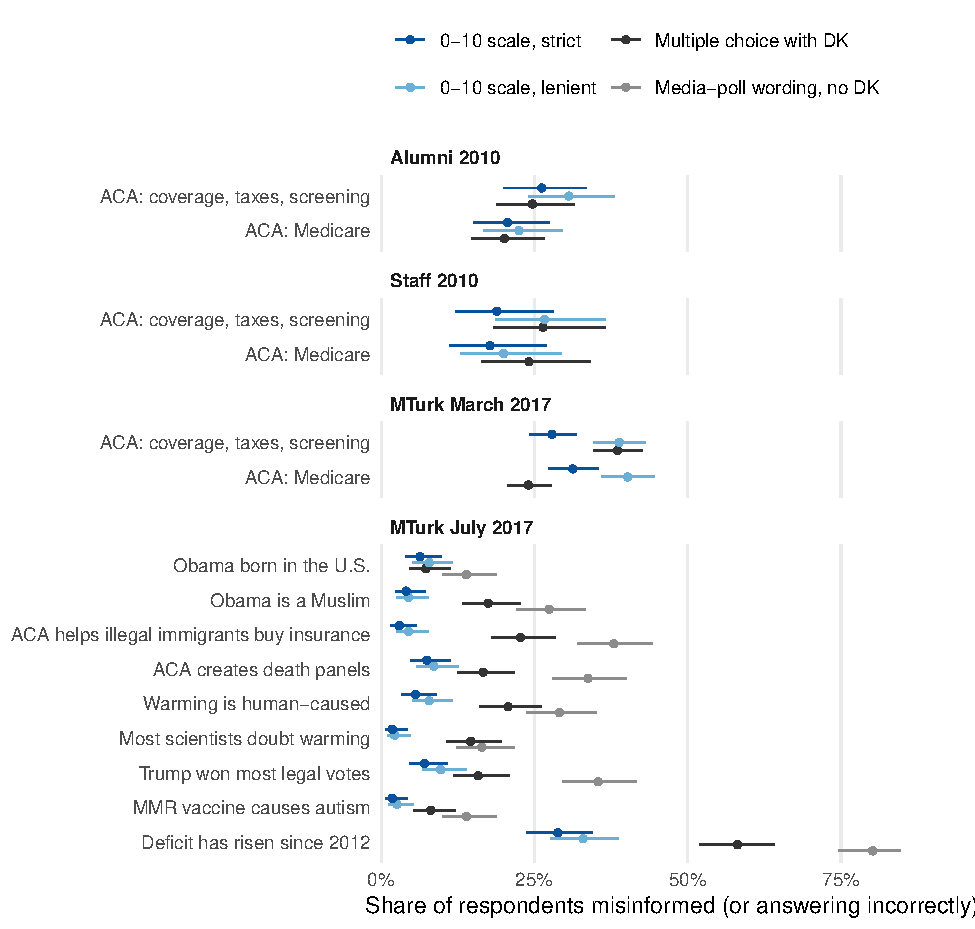
\includegraphics[width=\linewidth]{format.pdf}
\caption{Misinformation measured four ways. Points are shares of respondents in each randomly assigned arm; lines are 95\% Wilson intervals. For multiple choice, the share choosing an incorrect option (DK and skipped answers count as not incorrect). For the 0--10 scale, the share with a confidently wrong rating of any of the question's propositions (strict: 0 or 10; lenient: 0--1 or 9--10); skipped and not-applicable ratings count as not misinformed. Media-poll wording was asked only in July 2017.}
\label{fig:format}
\end{figure}

For the well-publicized falsehoods of the July survey, the scale finds far less misinformation than multiple choice does, and multiple choice with a DK option finds far less than media-poll wording. \muslimMedia{} of respondents said Obama is a Muslim when asked as media polls ask, \muslimMc{} when the question offered DK, and \muslimScale{} were confident of it on the scale. For the ACA and illegal immigrants, the three numbers are \illegalMedia{}, \illegalMc{}, and \illegalScale{}; for Trump's winning most legal votes, \fraudMedia{}, \fraudMc{}, and \fraudScale{}. Pooling the July questions, the scale lowers the share misinformed by \julyStrict{} percentage points relative to multiple choice with DK (95\% interval \julyStrictLower{} to \julyStrictUpper{}), from a base that is itself deflated by the DK option.

The deficit item is the exception that proves the measure is not merely deflationary. The federal deficit fell from \$1,087 billion in fiscal year 2012 to \$585 billion in 2016, yet \deficitScale{} rated ``the annual federal budget deficit has increased since 2012'' definitely true, against \deficitMc{} choosing ``increased'' or ``stayed about the same'' with a DK option and \deficitMedia{} with media wording. A plausible reading is stereotypic inference of the kind described above: deficits are large, the debt was rising, and ``increased'' is what deficits do.

For the obscurer provisions of the ACA, the formats differ little. In the 2010 surveys and in March 2017, the strict scale share is within a few points of the multiple-choice share (\alumniStrict{} points higher among alumni, \staffStrict{} lower among staff, \marchStrict{} lower in March), and the lenient scale share runs \marchLenient{} points higher in March. Two things explain the contrast with July. These multiple-choice items offered DK and drew many DKs, so their incorrect answers were already fewer; and each ACA question bundles four propositions, so the any-proposition rule gives the scale four chances to register misinformation to multiple choice's one. Across all questions and surveys, the scale finds \pooledStrict{} points less misinformation (95\% interval \pooledStrictLower{} to \pooledStrictUpper{}) under strict scoring and \pooledLenient{} points less under lenient scoring.

\subsection{Invention and Denial}

The scale separates invention from denial. For the ACA's lesser-known provisions, denial is the more common: \denialAlumni{} of alumni ratings of its true provisions (a Medicare payroll tax on high earners and limits on payments to Medicare providers) were confidently false, against \inventionAlumni{} of ratings of its false ones; among staff, \denialStaff{} and \inventionStaff{}; in March 2017, \denialMarch{} and \inventionMarch{}. For the better-known claims of the July survey, invention and denial are about equally common (\inventionJuly{} and \denialJuly{}). Confident disbelief in true but little-publicized provisions looks less like motivated rejection than like inference from what a law of that kind would do; it is a reminder that misinformation need not come from anyone's promoting it.

\subsection{Partisan Misinformation}

If the measure captures motivated misinformation, Republicans should be more misinformed about falsehoods congenial to them and Democrats about falsehoods congenial to them. Figure~\ref{fig:gaps} shows that they are. Of the \nRcongenial{} propositions in the two MTurk surveys whose errors favor Republicans, \nRpositive{} show more misinformation among Republicans (\nRclear{} with 95\% intervals excluding zero), and the \nDcongenial{} whose errors favor Democrats (among them that greenhouse gases cause lung cancer and that the executive order stripped green cards) show more among Democrats, though with wide intervals.

\begin{figure}[t]
\centering
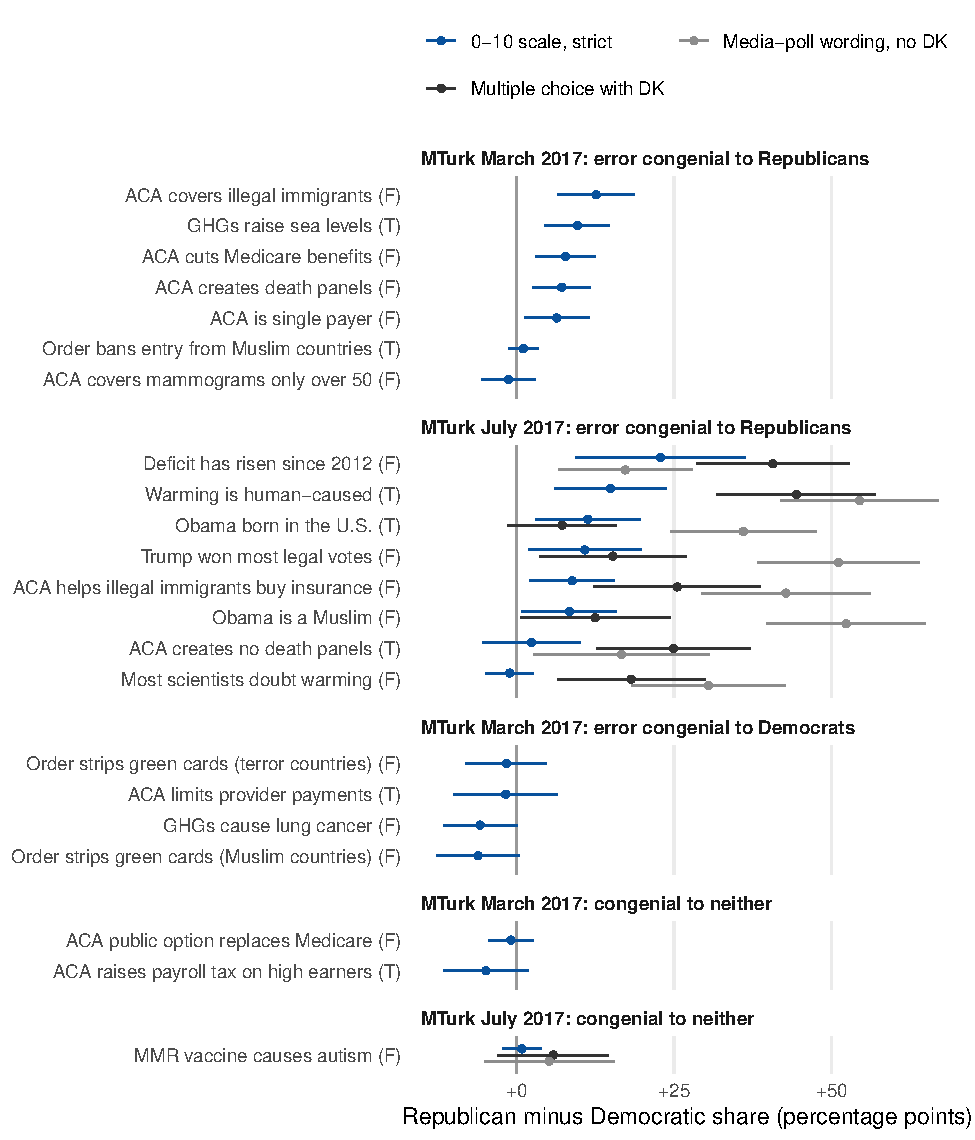
\includegraphics[width=\linewidth]{partisan_gaps.pdf}
\caption{Partisan gaps in misinformation. Points are Republican minus Democratic shares (with leaners) misinformed on the scale (strict scoring) or answering incorrectly on multiple choice; lines are 95\% intervals from unpooled binomial standard errors. T and F mark true and false statements; for true statements, misinformation is confident disbelief. Panels group statements by the party to which the error is congenial.}
\label{fig:gaps}
\end{figure}

The gaps are much smaller on the scale than in multiple-choice answers. Republicans were \gapMuslimMedia{} points more likely than Democrats to say Obama is a Muslim with media wording, \gapMuslimMc{} points with a DK option, and \gapMuslimScale{} points on the scale; for Trump's legal votes the gaps are \gapFraudMedia{}, \gapFraudMc{}, and \gapFraudScale{}. On whether warming is human-caused, the gap falls from \gapWarmingMc{} points to \gapWarmingScale{}, and on whether most scientists doubt warming from \gapScienceMc{} to \gapScienceScale{}. Much of the partisan gap in answers to misinformation items is thus not partisan misinformation but partisan guessing, inference, and cheerleading, in line with evidence that incentives and DK options shrink partisan gaps in factual answers \citep{bullock2015, prior2015, schaffner2018, peterson2021}. What remains is not trivial: \gapDeficitScale{} points on the deficit and double digits on Obama's birthplace, Trump's legal votes, and human-caused warming.

\subsection{Who Is Misinformed?}

The misinformed resemble the knowledgeable in one way the introduction anticipated: both are more interested in politics. Within the scale arms, moving from no interest to maximal interest raises the share of ratings at the correct end by \interestKnows{} points (standard error \interestKnowsSe{}) from an average of \meanKnows{}, and raises the share at the incorrect end by \interestMisinformed{} points (95\% interval \interestMisinformedLower{} to \interestMisinformedUpper{}) from an average of \meanMisinformed{}. Both estimates hold each proposition fixed and cluster standard errors by respondent. Interest brings confident belief, most of it right but some of it wrong.

\section{Discussion}

According to much news coverage and some scholarly literature, the American public is awash in misinformation. That picture, it now seems, is considerably overdrawn. There is misinformation, to be sure, but much less than the headlines suggest. Some of what masquerades as misinformation is guessing or inference---not pre-existing, stored cognition but on-the-spot processing, occasioned only by the task of answering the question. Some is pre-existing belief, just not confidently enough held to constitute misinformation. Much the same may be said of knowledge. There is some, but much less than the raw responses to questionnaire items suggest. Many correct responses, too, are the products of guessing, fresh inference, or mere belief. The besetting deficiency in public opinion is not misinformation but ignorance.

Even the scale's estimates are probably too high. \citet{graham2023} finds that people who say they are certain of a falsehood often give a different answer weeks later, at rates similar to those who say they are certain of obscure scientific falsehoods, and concludes that confident wrong answers are often miseducated guesses rather than stored beliefs. If so, some of what the scale counts as misinformation is confident inference made on the spot, and the true prevalence is lower still. The scale also inherits the respondent's use of it: people who reserve the endpoints for near certainty will register less knowledge and less misinformation than those who use them freely, and a single wave cannot tell those apart from genuine differences in confidence.

Two further limits bear on the comparisons. The samples are convenience samples, drawn from a university's alumni and staff and from MTurk, so the levels do not describe the public; the comparisons between randomly assigned formats within each survey are what the design identifies. And the keys are ours. We have tried to keep only propositions that are plainly true or plainly false and to document the basis for each, but the one we consider most debatable among those we keep---that the ACA cuts benefits to existing Medicare patients, which is false of guaranteed benefits but not of every extra benefit offered by private Medicare plans---shows how fine the line can be.

That said, misinformation exists and may be consequential. So, short of actual misinformation, may tentative mistaken belief. Much remains to be done in measuring them and examining their sources and consequences.

\bibliographystyle{apsr}
\bibliography{references}

\clearpage
\appendix
\section*{Appendix}
\setcounter{table}{0}
\renewcommand{\thetable}{A\arabic{table}}

\begin{table}[H]
\centering
\caption{Balance across randomly assigned arms}
\label{tab:balance}
\small
\begin{tabular}{llrrrr}
\toprule
Study & Arm & $n$ & Democrat & Republican & Interest (0--10) \\
\midrule
Alumni 2010 & Multiple choice with DK & 174 & 0.70 & 0.16 & 6.4 \\
 & 0--10 scale & 160 & 0.73 & 0.14 & 6.5 \\
Staff 2010 & Multiple choice with DK &  87 & 0.71 & 0.17 & 5.6 \\
 & 0--10 scale &  90 & 0.81 & 0.08 & 5.4 \\
MTurk March 2017 & Multiple choice with DK & 557 & 0.53 & 0.31 & 6.0 \\
 & 0--10 scale & 502 & 0.49 & 0.32 & 5.8 \\
MTurk July 2017 & Multiple choice with DK & 246 & 0.58 & 0.27 & 6.2 \\
 & Media-poll wording & 237 & 0.54 & 0.29 & 6.4 \\
 & 0--10 scale & 267 & 0.58 & 0.25 & 6.2 \\
\bottomrule
\end{tabular}

\begin{minipage}{0.8\linewidth}
\vspace{0.5em}\footnotesize \emph{Note:} Shares of respondents identifying with or leaning toward each party; mean political interest on a 0--10 scale.
\end{minipage}
\end{table}

\begin{table}[H]
\centering
\caption{Belief states on the 0--10 scale (strict scoring), percent of ratings}
\label{tab:states}
\footnotesize
\setlength{\tabcolsep}{2pt}
\begin{tabular}{llcrrrrrr}
\toprule
Study & Proposition &  & $n$ & Know & Lean right & 5 & Lean wrong & Misinf. \\
\midrule
Alumni 2010 & Covers illegal immigrants & F & 158 & 46 & 22 & 20 & 7 & 6 \\
 & Cuts Medicare benefits & F & 160 & 36 & 26 & 23 & 11 & 4 \\
 & Death panels & F & 160 & 59 & 15 & 14 & 9 & 2 \\
 & No mammograms under 50 & F & 157 & 24 & 19 & 38 & 11 & 8 \\
 & Public option replaces Medicare & F & 160 & 63 & 13 & 14 & 8 & 2 \\
 & Single payer & F & 159 & 71 & 12 & 10 & 6 & 1 \\
 & Limits provider payments & T & 159 & 5 & 33 & 35 & 11 & 16 \\
 & Raises payroll tax on high earners & T & 159 & 13 & 31 & 28 & 11 & 18 \\
Staff 2010 & Covers illegal immigrants & F &  89 & 46 & 16 & 22 & 13 & 2 \\
 & Cuts Medicare benefits & F &  90 & 37 & 31 & 14 & 11 & 7 \\
 & Death panels & F &  89 & 64 & 11 & 17 & 6 & 2 \\
 & No mammograms under 50 & F &  90 & 33 & 12 & 29 & 20 & 6 \\
 & Public option replaces Medicare & F &  90 & 60 & 13 & 19 & 7 & 1 \\
 & Single payer & F &  90 & 71 & 12 & 10 & 7 & 0 \\
 & Limits provider payments & T &  88 & 9 & 25 & 48 & 7 & 11 \\
 & Raises payroll tax on high earners & T &  88 & 11 & 30 & 39 & 7 & 14 \\
MTurk March 2017 & ACA covers illegal immigrants & F & 502 & 26 & 29 & 19 & 18 & 8 \\
 & ACA covers mammograms only over 50 & F & 502 & 18 & 20 & 30 & 27 & 5 \\
 & ACA creates death panels & F & 502 & 41 & 24 & 16 & 16 & 4 \\
 & ACA cuts Medicare benefits & F & 502 & 34 & 27 & 16 & 19 & 4 \\
 & ACA is single payer & F & 502 & 34 & 25 & 15 & 20 & 6 \\
 & ACA public option replaces Medicare & F & 502 & 36 & 27 & 13 & 19 & 5 \\
 & GHGs cause lung cancer & F & 502 & 18 & 28 & 19 & 25 & 11 \\
 & Order strips green cards (Muslim countries) & F & 502 & 23 & 21 & 12 & 28 & 15 \\
 & Order strips green cards (terror countries) & F & 502 & 25 & 24 & 14 & 24 & 13 \\
 & ACA limits provider payments & T & 502 & 4 & 28 & 24 & 21 & 23 \\
 & ACA raises payroll tax on high earners & T & 502 & 10 & 34 & 21 & 21 & 14 \\
 & GHGs raise sea levels & T & 502 & 37 & 35 & 13 & 9 & 7 \\
 & Order bans entry from Muslim countries & T & 502 & 60 & 30 & 4 & 4 & 2 \\
MTurk July 2017 & ACA helps illegal immigrants buy insurance & F & 154 & 34 & 27 & 10 & 23 & 5 \\
 & Deficit has risen since 2012 & F & 185 & 11 & 12 & 5 & 31 & 42 \\
 & MMR vaccine causes autism & F & 236 & 62 & 25 & 6 & 5 & 2 \\
 & Most scientists doubt warming & F & 255 & 66 & 22 & 5 & 5 & 2 \\
 & Obama is a Muslim & F & 232 & 68 & 17 & 3 & 7 & 5 \\
 & Trump won most legal votes & F & 249 & 63 & 15 & 4 & 11 & 8 \\
 & ACA creates no death panels & T & 152 & 49 & 22 & 5 & 11 & 13 \\
 & Obama born in the U.S. & T & 243 & 72 & 14 & 3 & 5 & 7 \\
 & Warming is human-caused & T & 249 & 47 & 35 & 4 & 8 & 6 \\
\bottomrule
\end{tabular}

\begin{minipage}{0.95\linewidth}
\vspace{0.5em}\footnotesize \emph{Note:} Ratings are recoded so that 10 is the correct end: knowledge is 10, misinformation 0, leaning right 6--9, leaning wrong 1--4. $n$ counts respondents who rated the statement. T and F mark true and false statements.
\end{minipage}
\end{table}

{\footnotesize
\setlength{\tabcolsep}{3pt}
\begin{longtable}{lp{4.8cm}lp{7cm}}
\caption{Statements, keys, and the basis for each key}\label{tab:propositions}\\
\toprule
Survey & Statement & Key & Basis \\
\midrule
\endfirsthead
\toprule
Survey & Statement & Key & Basis \\
\midrule
\endhead
\bottomrule
\endlastfoot
2010 & Provides coverage for people who are currently in the country illegally & false & ACA sec. 1312(f)(3) bars people not lawfully present from exchange coverage and credits \\
2010 & Replaces private health insurance with a ``single payer system'' & false & ACA builds on private insurance through exchanges; no single-payer provision \\
2010 & Increases the Medicare payroll tax for upper-income Americans & true & ACA sec. 9015: additional 0.9\% Hospital Insurance tax on wages above \$200,000 (\$250,000 joint) \\
2010 & Does not reimburse routine mammograms for women younger than 50 & false & ACA sec. 2713 requires coverage without cost sharing of HRSA-supported screenings; the 2009 USPSTF update was set aside for coverage, so screening from age 40 is covered \\
2010 & Allows a government panel to make decisions about end-of-life care for people on Medicare & false & No such panel in the law; PolitiFact 2009 Lie of the Year; Nyhan (2010) \\
2010 & Replaces Medicare with a ``public option'' & false & The public option was dropped from the enacted law, and it would not have replaced Medicare \\
2010 & Limits future increases in payments to Medicare providers & true & ACA sec. 3401 productivity adjustments to Medicare provider payment updates (CBO 2010) \\
2010 & Cuts benefits to existing Medicare patients & false & Guaranteed Medicare benefits are unchanged; lower Medicare Advantage payments could trim plans' extra benefits, which makes this the most debatable of the kept propositions \\
Mar 2017 & Provides coverage for people who are currently in the country illegally & false & ACA sec. 1312(f)(3) \\
Mar 2017 & Replaces private health insurance with a ``single payer system'' & false & No single-payer provision \\
Mar 2017 & Increases the Medicare payroll tax for upper-income Americans & true & ACA sec. 9015 \\
Mar 2017 & Reimburse routine mammograms only for women older than 50 & false & ACA sec. 2713; screening from age 40 covered \\
Mar 2017 & Creates government panels to make end-of-life decisions for people on Medicare & false & No such panel in the law \\
Mar 2017 & Replaces Medicare with a ``public option'' & false & Public option dropped from the enacted law \\
Mar 2017 & Limits future increases in payments to Medicare providers & true & ACA sec. 3401 \\
Mar 2017 & Cuts benefits to existing Medicare patients & false & Guaranteed benefits unchanged \\
Mar 2017 & A cause of respiratory problems & dropped & Dropped: ground-level ozone is both a greenhouse gas and a respiratory irritant \\
Mar 2017 & A cause of lung cancer & false & No major greenhouse gas (CO2, CH4, N2O, fluorinated gases) is a lung carcinogen; the carcinogens in combustion exhaust are co-pollutants \\
Mar 2017 & Damaging the ozone layer & dropped & Dropped: nitrous oxide and CFCs are greenhouse gases that deplete stratospheric ozone \\
Mar 2017 & A cause of rising sea levels & true & IPCC AR5 WG1 Summary for Policymakers (2013) \\
Mar 2017 & Unconnected to burning natural gas & dropped & Dropped with its question: a last-minute edit left two correct options \\
Mar 2017 & Produced more by burning clean coal than by other fossil fuels & dropped & Dropped with its question \\
Mar 2017 & Produced by nuclear power plants & dropped & Dropped with its question \\
Mar 2017 & Reduced by trees and other plants & dropped & Dropped with its question \\
Mar 2017 & Subjects immigrants living in the U.S. illegally to deportation & dropped & Dropped: the most recent order (EO 13780) did not, but the January interior-enforcement order (EO 13768) expanded removal priorities \\
Mar 2017 & Strips immigrants from countries supporting terrorism of their green cards & false & EO 13780 sec. 3(b)(i) exempts lawful permanent residents \\
Mar 2017 & Strips immigrants from several Muslim-majority countries of their green cards & false & EO 13780 sec. 3(b)(i) exempts lawful permanent residents \\
Mar 2017 & Temporarily bans immigrants from several majority-Muslim countries & true & EO 13780 sec. 2(c) suspends entry from six majority-Muslim countries for 90 days \\
Jul 2017 & Barack Obama was born in the US & true & Hawaii State Department of Health birth certificate (2011) \\
Jul 2017 & Barack Obama is a Muslim & false & Obama is a Christian (Pew Research Center 2010) \\
Jul 2017 & The Affordable Care Act gives illegal immigrants financial help to buy health insurance & false & ACA sec. 1312(f)(3) \\
Jul 2017 & The Affordable Care Act does not create government panels to make decisions about end-of-life care & true & No such panel in the law \\
Jul 2017 & Temperatures around the world are increasing because of human activity, like burning coal and gasoline & true & IPCC AR5 WG1 Summary for Policymakers (2013) \\
Jul 2017 & Most climate scientists believe that global warming is not occurring & false & Cook et al. (2016) \\
Jul 2017 & In the 2016 presidential election, President Trump won the majority of the legally cast votes & false & FEC official 2016 results: Trump won 46.1\% of votes cast, so he would hold a majority of legal votes only if more than 10 million votes for other candidates were illegal \\
Jul 2017 & The vaccine for measles, mumps, and rubella (MMR) causes autism in children & false & Taylor, Swerdfeger and Eslick (2014) \\
Jul 2017 & Since 2012, the annual federal budget deficit has increased & false & CBO: deficit \$1,087 billion in FY2012, \$585 billion in FY2016 \\
\end{longtable}

}

\end{document}
